\problemname{Alien Language}
\begin{center}
    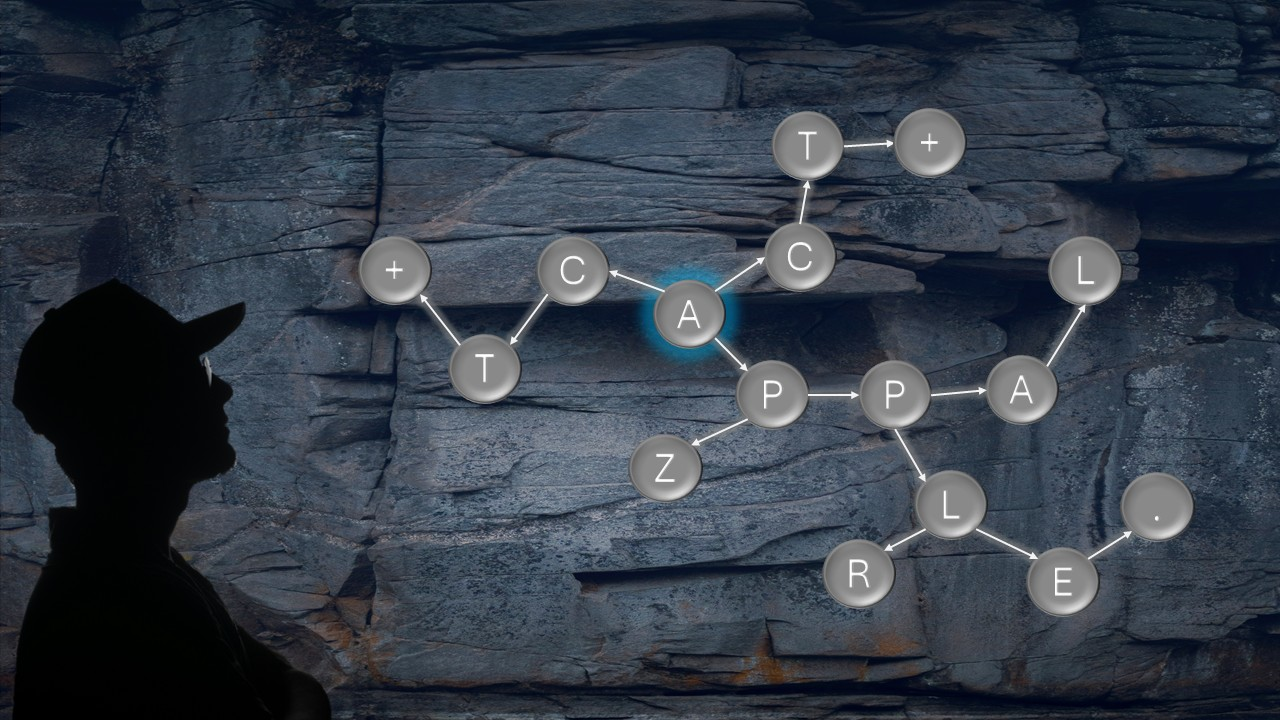
\includegraphics[width=1\textwidth]{images/problem.jpg}
\end{center}

\definecolor{codebg}{gray}{0.92}
\newcommand{\code}[1]{%
    {\setlength{\fboxsep}{1.5pt}\colorbox{codebg}{\texttt{\strut #1}}}%
}

\begin{flushleft}
    "Sco bo tro no flo jo ko fo to do. No bo ho sho ko ro to so. Bokodozogobofopojo. Ma ho."
\end{flushleft}

\begin{flushright}
    --- Famous alien from a Blue Box, 2008. \\
\end{flushright}

\begin{flushleft}
    You are a translator sent out into deep space to study a new alien language. You have landed on the planet and began surveying. Deep inside the cave of the planet, you come across a cave wall with a glowing letter with arrows that extend out to other letters. You decide to call these graph words and the glowing letter as the source. \\
\end{flushleft}

\begin{flushleft}
    A graph word(\textbf{GW}) is a word that starts from the source and ends at the sink with no further leaves. Example, \code{ACT+}, \code{APZ} and \code{APPLE.} is a graph word. \code{APPA} or \code{ACT} are not graph words. \\
\end{flushleft}

\begin{flushleft}
    A graph word can have modifiers which are \code{.} and \code{+}. There is only one GW with the modifier \code{.} but there are multiple GWs with the modifier \code{+}. Example 1, \code{ACT+} can be broken down into \code{ACT} with the modifier \code{+}. Example 2, \code{APPLE.} can be broken down into \code{APPLE} with the modifier \code{.}. Example 3, \code{APZ} cannot be broken down further and has no modifier. \\
\end{flushleft}

\begin{flushleft}
    As a translator, you are given a dictionary similar to an Oxford English Dictionary. The first dictionary word(\textbf{DW}) is blank which means the following DWs begin with an index of 1. A GW can be verified using the dictionary if a GW exists in the dictionary. Once the GW is verified, the GW is considered a valid word and you can access the index from the dictionary. \\
\end{flushleft}

\begin{flushleft}
    Example 1, in a dictionary with the DWs of \code{[ACT, APPLE, APZ]}, a GW of \code{ACT+} is a valid DW and returns the index of 1. Example 2, in a dictionary with the DWs of \code{[ACT, APPLE, APZ]}, a GW of \code{APPLE.} is a valid DW and returns the index of 2. Example 3, in a dictionary with the DWs of \code{[ACT, APPLE, APZ]}, a GW of \code{APZ} is a valid DW and returns the index of 3.\\
\end{flushleft}

\begin{flushleft}
    There is one problem, your radio antenna has low bandwidth which means simply sending the word back to Earth will take too long. You will have to send back a coded message. \\
\end{flushleft}

\begin{flushleft}
    The \textbf{coded message} is made of 3 lines:
    \begin{itemize}
        \item The \textit{first line} is the sum of indices of valid GWs with the modifier \code{+}. Otherwise, return 0.

        \item The \textit{second line} is a sorted list of indices of all valid GWs regardless of modifiers. Otherwise, return nothing.

        \item The \textit{third line} is the index of the valid GW that ends with \code{.}. Otherwise, return nothing.
    \end{itemize}
\end{flushleft}

\section*{Input}

\begin{flushleft}
    The first line contains N, R, D ($1 \leq N \leq 500,000$, $1 \leq R \leq 500,000$, $1 \leq D \leq 500,000$) where N is the number of nodes, R is the number of relations, D is the number of DWs in the dictionary. \\
\end{flushleft}

\begin{flushleft}
    The second line contains the DWs in the dictionary. The third line contains the start node and the letter of the alphabet. \\
\end{flushleft}

\begin{flushleft}
    The following lines are based on the number of relations where Line A (for A = 0, 1, ..., R - 1) has 3 values. The values are source node, destination node and letter / modifier (\code{.} or \code{+}).
\end{flushleft}

\section*{Output}
\begin{flushleft}
    Output a coded message.
\end{flushleft}
